\documentclass[]{beamer}
\usepackage{lmodern}
\usepackage{datetime}
\usepackage{wrapfig}
\usepackage{tikz}
\usetikzlibrary{arrows,shapes}

\renewcommand\mathfamilydefault{\rmdefault}


\usetheme{Boadilla}

% ---- Editing the footer --------
\makeatother
\setbeamertemplate{footline}
{
  \leavevmode%
  \hbox{%
  \begin{beamercolorbox}[wd=.4\paperwidth,ht=2.25ex,dp=1ex,center]{institute in head/foot}%
    \usebeamerfont{institute in head/foot}\insertshortinstitute
  \end{beamercolorbox}%
  \begin{beamercolorbox}[wd=.6\paperwidth,ht=2.25ex,dp=1ex,center]{date in head/foot}%
    \usebeamerfont{date in head/foot}\insertshortdate\hspace*{2em}
     \insertframenumber{} / \inserttotalframenumber\hspace*{2ex}
  \end{beamercolorbox}}%
  \vskip0pt%
}
\makeatletter
\setbeamertemplate{navigation symbols}{}
% --------------------------------------

% ------ Date definition ------------------
\newdate{date}{9}{9}{2014}
% -----------------------------------------

\title{Solving the guiding center model using the Semi-Lagrangian scheme on a 2D hexagonal mesh (SelHex)}  
\author{Michel Mehrenberger, Laura Mendoza, Charles Prouveur,\\ Eric Sonnendr\"{u}cker}
\institute[SelHex (CEMRACS 2014)]
{
}\date{\displaydate{date}} 


%%%%%%%%%%%%%%%%%%%%%%%%%%%%
\begin{document}

\begin{frame}
\titlepage
\end{frame} 


\begin{frame}
\frametitle{Table of contents}
\tableofcontents
\end{frame} 


\section{Motivation} 


\begin{frame}
	\frametitle{Motivation}
	\begin{columns}
    	\begin{column}{0.45\textwidth}
    		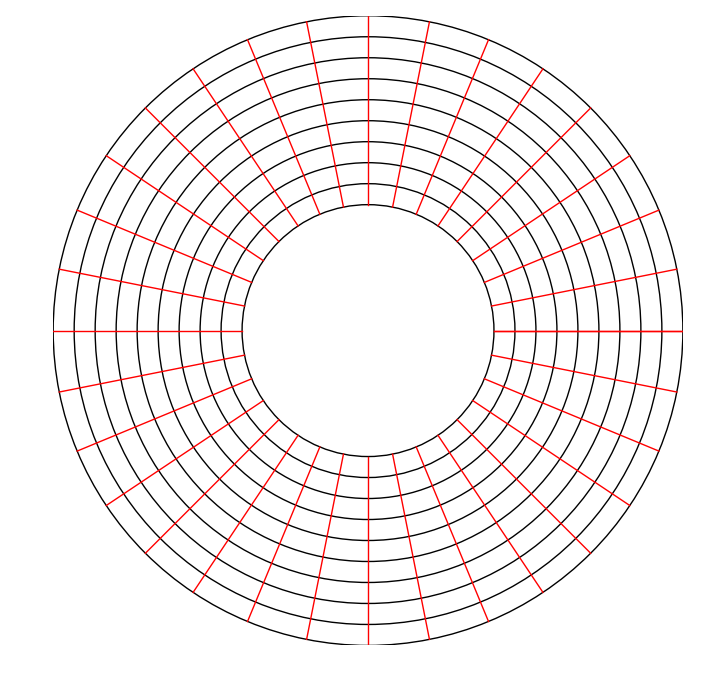
\includegraphics[width=1.0\textwidth]{mapping.png}
    	\end{column}
    	\begin{column}{0.5\textwidth}
    		Current representation of the poloidal plane :
    		\begin{itemize}
    	    		\item Annular geometry
    			\item \textbf{Polar mesh} $(r, \theta)$
   		 \end{itemize}
   	 	Some limitations of this choice :
    		\begin{itemize}
    			\item{Geometric (and numeric)  \textbf{singular point} at origin of mesh}
    			\item{Unrepresented area and very costly to minimize that area}
    			\item{Impossible to represent \textbf{complex geometries} }
    		\end{itemize}
    	\end{column}
	\end{columns}
\end{frame}



\section{The hexagonal mesh} 
\begin{frame}
	\frametitle{The hexagonal mesh}

	\textbf{Idea:} Use a new mapping: hexagon $\longrightarrow$ circle.

	We define a tiling of triangles of a hexagon as our mesh for a 2D poloidal plane.

	\begin{columns}
    		\begin{column}{0.45\textwidth}

	\begin{figure}[h!]
	\begin{center} 
	\begin{tabular}{ccc}
	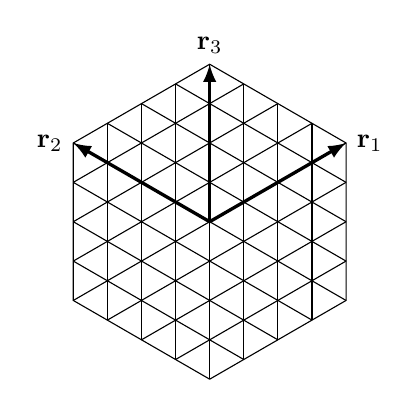
\begin{tikzpicture}

	% Three directions of grid
	\draw [-latex, very thick] (0, 0) -- (0,2) node(yline)[above] {$\mathbf{r}_3$};
	\draw [-latex, very thick] (0, 0)  -- (1.732,1) node(yline)[right] {$\mathbf{r}_1$} ;
	\draw [-latex, very thick] (0, 0) -- (-1.732,1) node(yline)[left] {$\mathbf{r}_2$};
	% vertical direction
	\draw (0,-2) -- (0,2);
	\draw (-0.433,-1.75) -- (-0.433,1.75);
	\draw (-0.866,-1.5) -- (-0.866,1.5);
	\draw (-1.3,-1.25) -- (-1.3,1.25);
	\draw (0.433,-1.75) -- (0.433,1.75);
	\draw (0.866,-1.5) -- (0.866,1.5);
	\draw (1.3,-1.25) -- (1.3,1.25);
	% upward
	\draw(-1.732,-1) -- (1.732,1);
	\draw (-1.732,-.5) -- (1.3,1.25);
	\draw (-1.732,0) -- (.866,1.5);
	\draw (-1.732,.5) -- (.433,1.75);
	\draw (-1.3,-1.25) -- (1.732,.5); 
	\draw (-0.866,-1.5) -- (1.732,.0);
	\draw (-0.433,-1.75) -- (1.732,-.5);
	% downwards
	\draw(-1.732,1) -- (1.732,-1);
	\draw (-1.732,.5) -- (1.3,-1.25);
	\draw (-1.732,0) -- (.866,-1.5);
	\draw (-1.732,-.5) -- (.433,-1.75);
	\draw (-1.3,1.25) -- (1.732,-.5); 
	\draw (-0.866,1.5) -- (1.732,.0);
	\draw (-0.433,1.75) -- (1.732,.5);
	% Hexagog
	\draw (0,-2) -- (1.732,-1) -- (1.732,1) -- (0,2) -- (-1.732,1) -- (-1.732,-1) -- (0,-2) ; % size 2

	\end{tikzpicture}
	\end{tabular}
	\end{center}
	\end{figure}

    \end{column}
    \begin{column}{0.5\textwidth}
   	Some advantages:
    	\begin{itemize}
	    	 \item No singular points
		\item (Hopefully) no need of multiple patches for the core of the tokamak
		\item Twelve-fold symmetry $\Rightarrow$ more efficient programming
		\item Easy transformation from cartesian to hexagonal coordinates
		\item Easy mapping to a disk
    	\end{itemize}
    \end{column}
\end{columns}

\end{frame}




\section{The Semi-Lagrangian Method} 
\begin{frame}
	\frametitle{The Backward Semi-Lagrangian Method}

	We consider the advection equation\vspace{-0.2cm}

	\begin{equation}
		\dfrac{\partial f}{\partial t} + \mathbf{a} (x, t) \cdot \nabla_\mathbf{x} f = 0
	\end{equation}\vspace{-0.5cm}

	\textbf{The scheme:}

	\begin{itemize}
		\item Fixed grid on phase-space
		\item Method of characteristics : ODE $\longrightarrow$ origin of characteristics
		\item Density $f$ is conserved along the characteristics
			\begin{equation}
			\text{\it{i.e.}} \quad \quad f^{n+1}(\mathbf{x}_i) = f^n(X(t_n; \mathbf{x}_i, t_{n+1}))
			\end{equation}
		\item Interpolate on the origin using known values of previous step at mesh points (initial distribution $f^0$ known).
	\end{itemize}

	\begin{center}
    		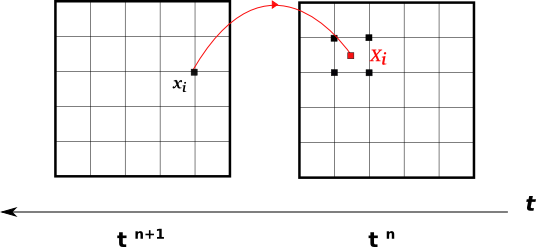
\includegraphics[width = 0.45\textwidth]{SL.png}
	\end{center}
\end{frame}


\section{The Guiding Center model} 
\begin{frame}
	\frametitle{The guiding center model: general algorithm}

	We consider a reduced model of the gyrokinetic model -- a simplified 2D Vlasov equation coupled with Poisson--:  
	
	\begin{equation}
	\left\{
	\begin{array}{lr}
	\dfrac{\partial f}{\partial t} + E_{\perp} \cdot \nabla_X f = 0\\
	- \Delta \phi = f
	\end{array}
	\right.
	\end{equation}
	
	\textbf{The global scheme:}

	\begin{itemize}
		\item Known: initial distribution function $f^0$ and electric field $E^0$
		\item Solve (Leap frog, RK4, ...) ODE for origin of characteristics $X$
		\item For every time step :
			\begin{itemize}
				\item Solve poisson equation $\Rightarrow E^{n+1}$
				\item Interpolate distribution in $X^{n}$ $\Rightarrow f^{n+1}$
			\end{itemize}
	\end{itemize}

\textbf{Two different approaches for interpolation step:} 

Spline and Hermite Finite Elements interpolations.

\end{frame}


\subsection{First approach: Splines interpolation}
\begin{frame}
	\frametitle{First approach: B(asis)-Splines basis*}

	B-Splines of degree $d$ are defined by the \textbf{recursion} formula: 

	\begin{equation}
	B_j^{d+1}(x)= \dfrac{x - x_j}{x_{j+d}-x_j} B_j^d(x)+ \dfrac{x_{j+1} - x}{x_{j+d+1} - x_{j+1}} B_{j+1}^d (x)
	\end{equation}

	Some important properties about B-splines:

	\begin{itemize}
		\item Piecewise polynomials of degree $d \quad \Rightarrow$ \textbf{smoothness} 
		\item Compact support $\Rightarrow$ \textbf{sparse matrix system}
		\item Partition of unity $\sum_j Bj (x) = 1$, $\forall x \quad \Rightarrow$ \textbf{conservation laws}
	\end{itemize}

	\begin{center}
		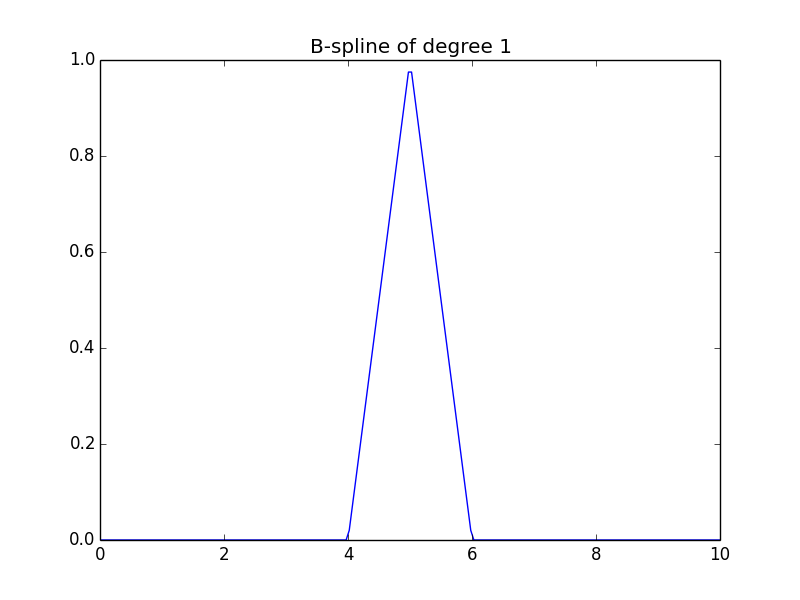
\includegraphics[width = 0.3\textwidth]{bsplines1.png}
		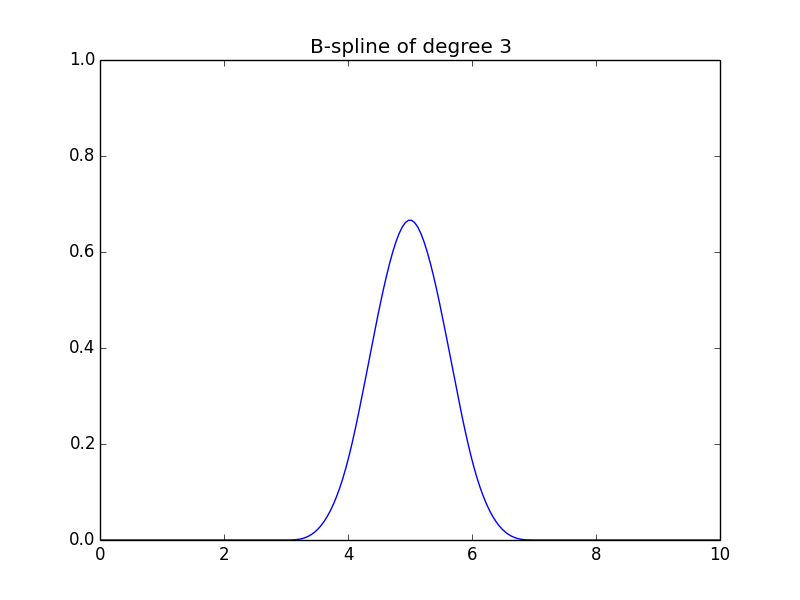
\includegraphics[width = 0.3\textwidth]{bsplines3.png}
		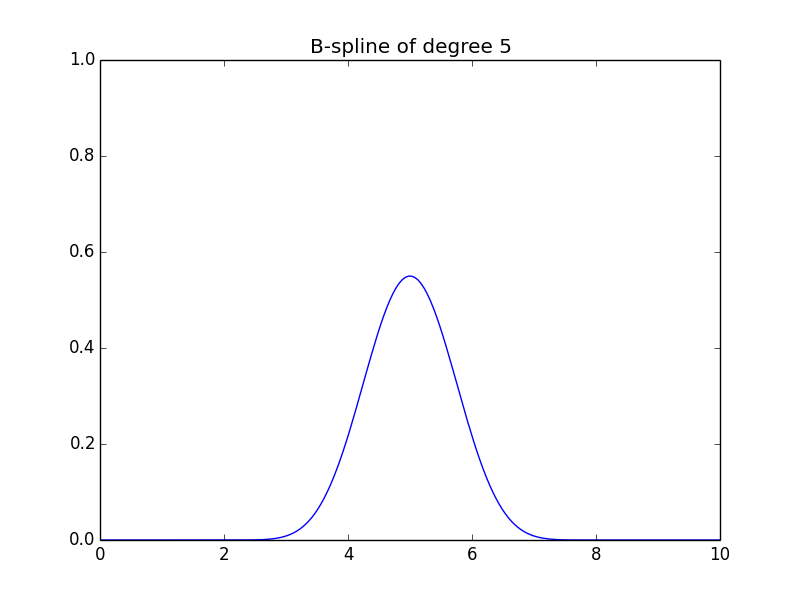
\includegraphics[width = 0.3\textwidth]{bsplines5.png}
	\end{center}

\end{frame}

\begin{frame}
	\frametitle{First approach: Box-splines and quasi-interpolation}
	\textbf{Box-Splines:}
	\begin{itemize}
		\item	Generalization of B-Splines
		\item Depend on the vectors that define the mesh
		\item Easy to exploit symmetry of the domain\vspace{0.2cm}
	\end{itemize}
	
	$\Rightarrow$ More efficient interpolation\vspace{0.2cm}

	\textbf{Quasi-interpolation:}
	\begin{itemize}
		\item Distribution function known at mesh points
		\item Of order $L$ if perfect reconstruction of a polynomial of degree $L - 1$
		\item No exact interpolation at mesh points $f_h(x_i) =  f(x_i)+O(\|x_i\| ^L)$\vspace{0.2cm}
	\end{itemize}
	
	$\Rightarrow$ Additional freedom to choose the coefficients $c_j$

	\begin{equation}
	f_h (x) = \sum c_j \chi^L (x - x_j)
	\end{equation}
\end{frame}


\subsection{Second approach: Hermite finite elements}

\begin{frame}{Second approach: Hermite finite elements}

Computed from the value of the function and its derivatives in various directions at various points.
	
Five in total have been implemented and tested:
    \hspace*{1.cm}
   		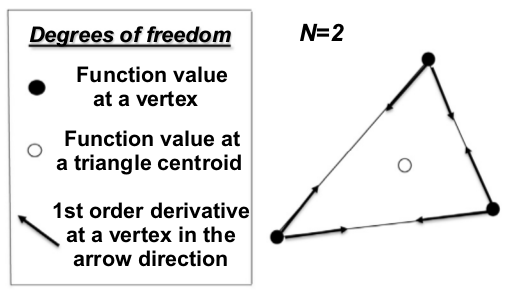
\includegraphics[width=0.4\textwidth]{z9.png}\\
    \hspace*{1.0cm}
   		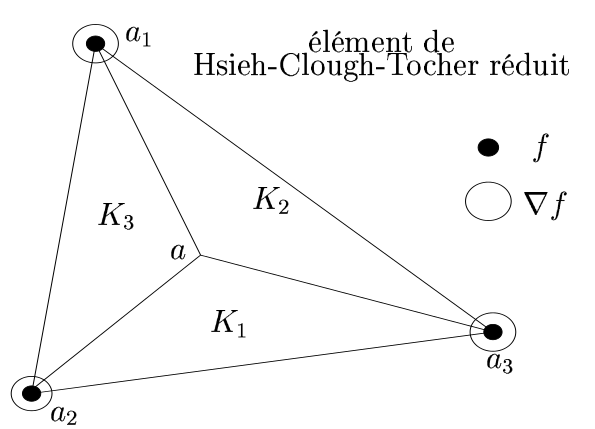
\includegraphics[width=0.25\textwidth]{hctr.png}
   		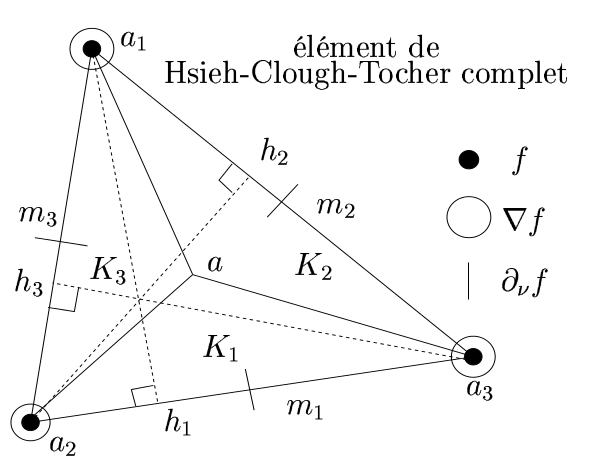
\includegraphics[width=0.25\textwidth]{hctc.png}
   		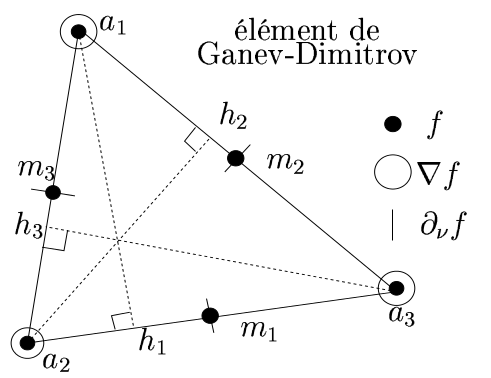
\includegraphics[width=0.25\textwidth]{ganev_dimitrov.png}

%5 were tested :
%  \begin{enumerate}
%  \item[-] Triangles de Zienkiewicz with 9 and 10 degrees of freedom
%  \item[-] Hsieh_Clough_Tocher_reduced and complete 9 and 12 degrees of freedom
%  \item[-] Ganev-Dimitrov element : 15 degrees of freedom
%  \end{enumerate}
% Triangles de Zienkiewicz with 9 and 10 degrees of freedom\\
% Hsieh_Clough_Tocher_reduced and complete \\
% (9 and 12 degrees of freedom)\\
% Ganev-Dimitrov element : 15 degrees of freedom\\	
\end{frame}


\begin{frame}
	\frametitle{Circular advection test case}
	
	In order to compare the two families' performances:
	\begin{equation}
		\partial_t f + y\partial_x f - x \partial_y f = 0 
	\end{equation}
	
	Taking a gaussian pulse as an initial distribution function
	\begin{equation}
	 f^{n} = exp  \left( -\dfrac{1}{2} \left( \dfrac{(x^n - x_c)^2}{\sigma_x^2} + \dfrac{(y^n - y_c)^2}{\sigma_y^2  } \right)   \right ) 
	\end{equation}
	Constant CFL (	$CFL = 2$ )  ,  $\sigma_x = \sigma_y = \frac{1}{2\sqrt{2}}$ , hexagonal radius : 8. \\
	Null Dirichlet boundary condition .
	
\end{frame}
\begin{frame}

	\textbf{Box-splines ($deg  = 2$) scheme:}
	\begin{center}
	\begin{tabular}{|c|c|c|c|c|c|c|}
		\hline
		 \textbf{Points} & \textbf{dt} & \textbf{loops}  & $L_2$ \textbf{error} & $L_\infty $ \textbf{error} & points/$\mu$-seconds \\
		\hline
		40   & 0.5         & 60   & 3.53E-2 & 7.74E-2  & 0.105 \\
		80   & 0.025    & 120 & 1.88E-3 & 4.66E-3 & 0.105 \\
		160 & 0.0125 & 240  & 6.77E-5 & 1.35E-4 & 0.105 \\
		\hline
	\end{tabular}
	\end{center}
	
	\textbf{Hermite FE scheme:}
	\begin{center}
	\begin{tabular}{|c|c|c|c|c|c|c|}
		\hline
		 \textbf{Points} & \textbf{dt} & \textbf{loops} & \textbf{CFL} & $L_2$ \textbf{error} & $L_\infty $ \textbf{error} & points/$\mu$-seconds \\
		\hline
		%20   & dt & numloops  & error1 & error2 & seconds  \\
		40   & dt & numloops & 1.28E-2 & error2  & seconds \\
		%60   & dt & numloops & error1 & error2 & seconds \\
		80   & dt & numloops & 3.43E-4& error2 & seconds \\
		%100 & dt & numloops & error1 & error2  & seconds\\
		%120 & dt & numloops  & error1 & error2  & seconds \\
		%140 & dt & numloops  & error1 & error2  & seconds\\
		160 & dt & numloops & 6E-6 & error2  & seconds \\
		\hline
	\end{tabular}
	\end{center}

\end{frame}

\begin{frame}{Circular advection: results 1}

    \hspace*{2.cm}
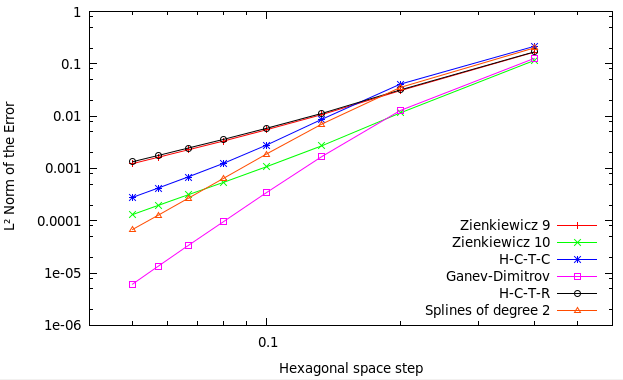
\includegraphics[width=0.55\textwidth]{l2.png}\\
    \hspace*{2.cm}
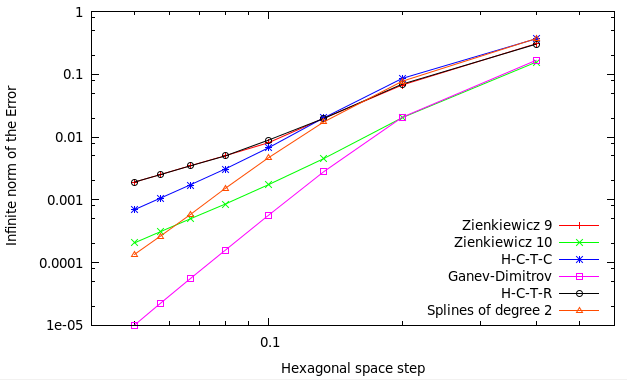
\includegraphics[width=0.55\textwidth]{inf_l.png}
\end{frame}
%
%\begin{frame}
%	\frametitle{Circular advection : results}
%	
%	Taking the dichotron distribution function
%	\begin{equation}
%	f^{n} = ...
%	\end{equation}
%	
%	\textbf{Splines scheme:}
%	\begin{center}
%	\begin{tabular}{|c|c|c|c|c|c|c|}
%		\hline
%		 \textbf{Points} & \textbf{dt} & \textbf{loops} & \textbf{CFL} & $L_2$ \textbf{error} & $L_\infty $ \textbf{error} & time \\
%		\hline
%		%20   & dt & numloops & CFL & error1 & error2 & seconds  \\
%		40   & dt & numloops & CFL & error1 & error2  & seconds \\
%		%60   & dt & numloops & CFL & error1 & error2 & seconds \\
%		80   & dt & numloops & CFL & error1 & error2 & seconds \\
%		%100 & dt & numloops & CFL & error1 & error2  & seconds\\
%		%120 & dt & numloops & CFL & error1 & error2  & seconds \\
%		%140 & dt & numloops & CFL & error1 & error2  & seconds\\
%		160 & dt & numloops & CFL & error1 & error2  & seconds \\
%		\hline
%	\end{tabular}
%	\end{center}
%	
%	\textbf{Hermite FE scheme:}
%	\begin{center}
%	\begin{tabular}{|c|c|c|c|c|c|c|}
%		\hline
%		 \textbf{Points} & \textbf{dt} & \textbf{loops} & \textbf{CFL} & $L_2$ \textbf{error} & $L_\infty $ \textbf{error} & time \\
%		\hline
%		%20   & dt & numloops & CFL & error1 & error2 & seconds  \\
%		40   & dt & numloops & CFL & error1 & error2  & seconds \\
%		%60   & dt & numloops & CFL & error1 & error2 & seconds \\
%		80   & dt & numloops & CFL & error1 & error2 & seconds \\
%		%100 & dt & numloops & CFL & error1 & error2  & seconds\\
%		%120 & dt & numloops & CFL & error1 & error2  & seconds \\
%		%140 & dt & numloops & CFL & error1 & error2  & seconds\\
%		160 & dt & numloops & CFL & error1 & error2  & seconds \\
%		\hline
%	\end{tabular}
%	\end{center}
%
%\end{frame}


\begin{frame}{Circular advection: results 2}

    \hspace*{2.cm}
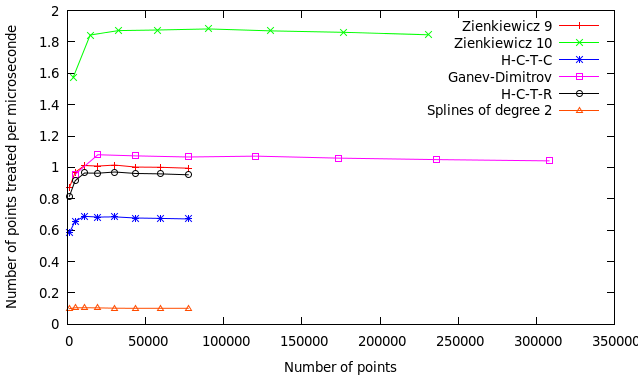
\includegraphics[width=0.55\textwidth]{efficiency.png}\\
    \hspace*{2.cm}
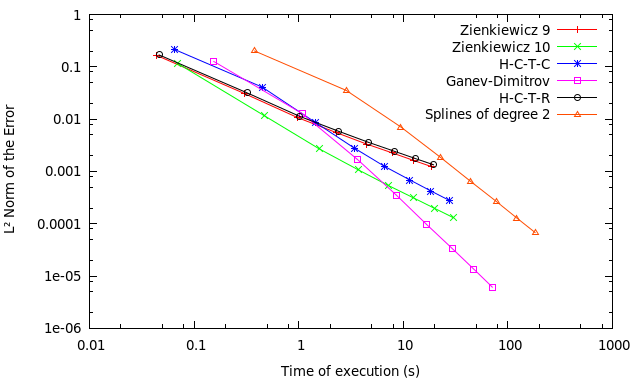
\includegraphics[width=0.55\textwidth]{time_norm.png}

\end{frame}

\section{Conclusion and perspectives}
\begin{frame}
	\frametitle{Conclusion and perspectives}

	\begin{itemize}
	 \item \textbf{Hexagonal mesh for SELALIB}	
	 \item \textbf{Comparison between two families of finite elements.} \\
	 \item[] 	Splines : good precision but poor efficiency.   	
	\item[] 	Amongst the other tested elements the complete Zienkiewicz's one seems to be the best choice in this case, at the moment.  
	
\item \textbf{Perspectives}
	 \begin{itemize}
	 \item[] Optimization.
	 \item[] Abstract classes.
	 \item[] Finite element solver of Poisson's equation on hexagonal mesh.
	\end{itemize}
	
	\end{itemize}
\end{frame}

\end{document}

